\label{Chapter1}

\chapter{Introduction}

\section{Motivation}
A space exploration vehicle designed to move across the surface of a planet,
besides Earth, is called a planetary rover as of its ability to "rove over"
an unknown terrain.
Planetary rovers are used to collect valuable data and samples such as
pictures, dust and rocks, which are later analyzed by scientists to enrich
our understanding regarding the universe.

Past missions have sent robots to the Moon and Mars (Figure
\ref{fig:mars_sites}) with the NASA's Curiosity being the last rover to
land on Mars in 2011.
Future missions do not differ much, as new lunar rovers are about to launch
in the next years and Mars rovers are currently under development scheduled
to be sent to Mars in 2020.

Such missions utilize a great amount of time and effort to build,
launch and finally operate.
Our interest lies in the operation challenges that are caused by the fact
that no constant communication can be achieved.
As an example, commanding messages can take up to 21 minutes to travel
between the Earth and Mars and bandwidth limitations can limit the number
of messages that can be sent.
This compounded to the unpredictable and unsafe conditions of
an unknown terrain such as the Mars surface which is full of rocks,
could lead to destructive system crashes of a costly mission.

Thus, we emphasize the need of a real time platform that will provide the
capability of autonomous operation with low supervision from ground control
as far as navigation is concerned.

\begin{figure}[h!]
    \centering
    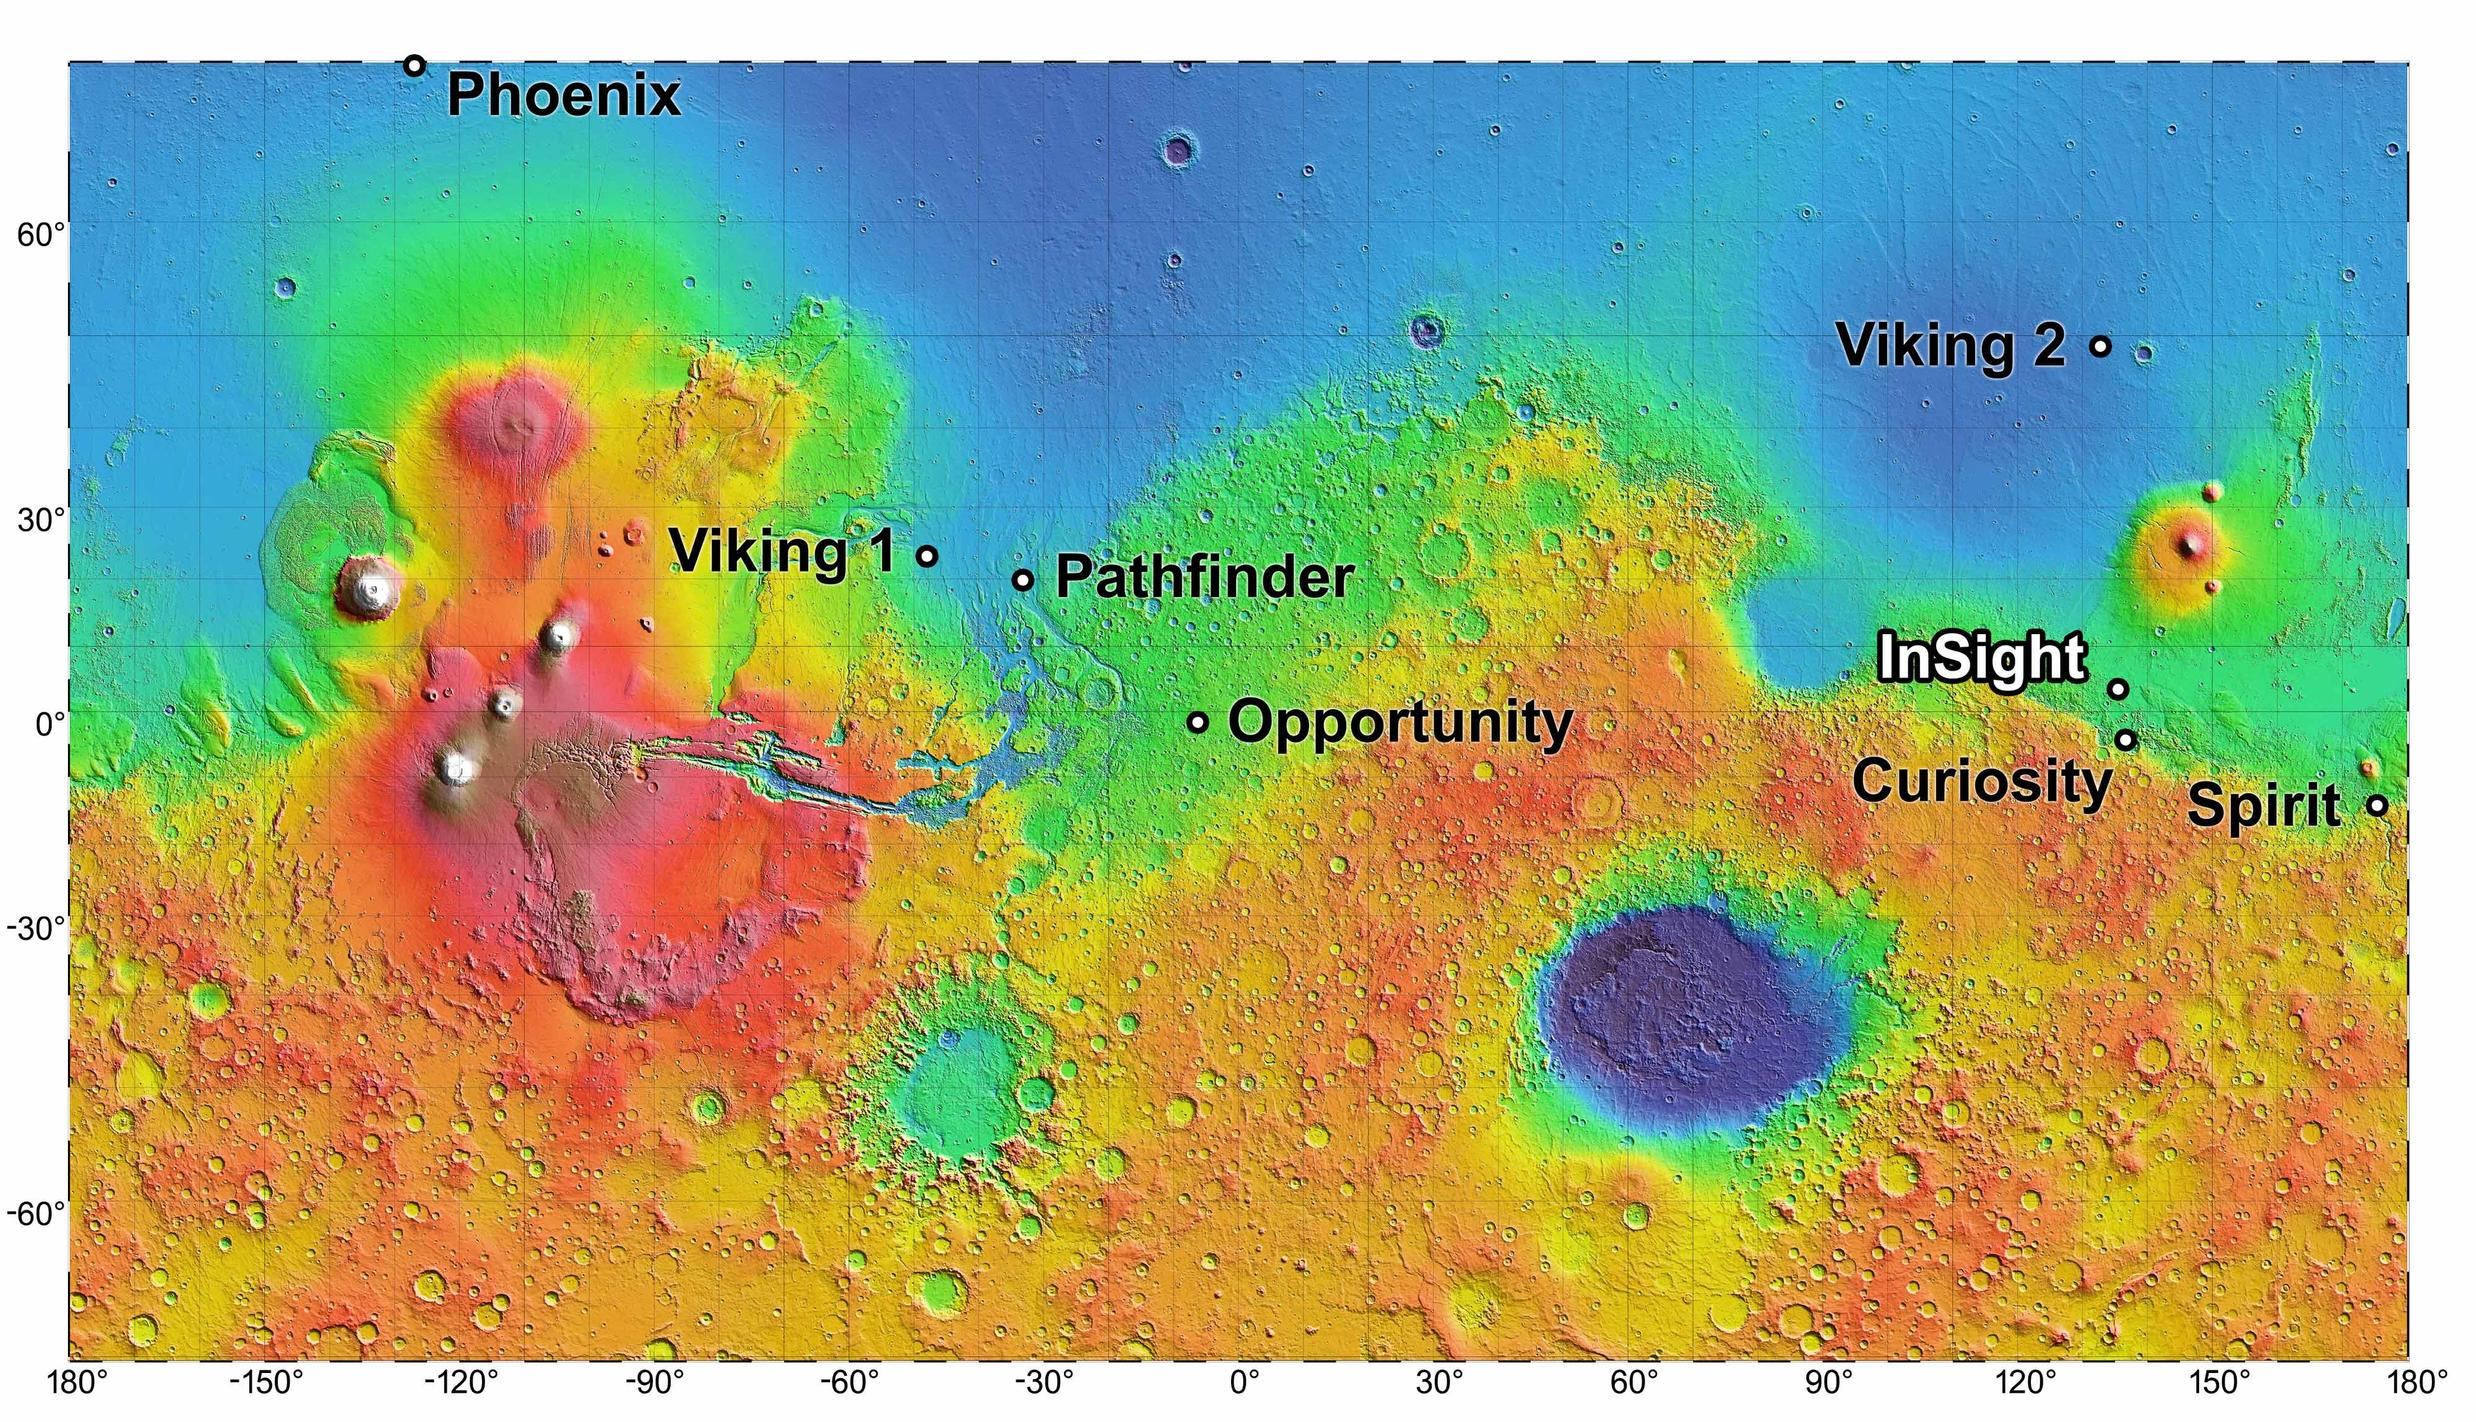
\includegraphics[scale=0.15]{mars_sites}
    \decoRule
    \caption[Mars landing sites]{
        Mars landing sites of rovers and landers from NASA's past missions.
    }
    \label{fig:mars_sites}
\end{figure}

\section{Problem Statement}

In order to navigate autonomously in extreme terrains, rovers need to
accurately perceive the 3D environment around them based on sensory
information.
Terrains that classify as extreme are areas with high variance in elevation
and great morphological anomalies, such as rocks and craters.

This thesis actively researches the challenges of perception in such terrains
in a planetary context and mainly focuses on two problems.
The first is the relative localization of the robot and the local mapping
of its surroundings in order to provide autonomous navigation capabilities
to it.
The second problem is the global localization of the robot, which is the
elimination of the accumulated drift from relative localization in long
range scenarios.

Specifically, given as inputs:
\begin{enumerate*}[label=(\roman*)]
    \item an initial prediction about the robot's movement,
    \item a detailed 3D representation of the close surroundings of the robot
        and
    \item an a priori low resolution map of the greater area,
\end{enumerate*}
the purpose is to output:
\begin{enumerate*}[label=(\roman*)]
    \item an accurate estimation of the position and orientation of the
        robot in a global reference frame and
    \item a local (robot-centric) map that represents the height of
        the environment.
\end{enumerate*}

\subsection{Presumptions}

In order to tackle the aspect of the problem that is of most interest,
we first assume the following:

\begin{itemize}
    \item a low resolution global map is available to the system at any time
    \item the initial global position of the robot is known
    \item the environment is static, i.e. is does not contain any
        moving objects
    \item the environment is unknown, i.e. there are no high resolution
        a priori maps available
    \item the terrain is single layered, i.e. there are no bridges or caves
\end{itemize}

\section{Literature Review}

\subsection{Simultaneous Localization and Mapping}

In early robotics research, localization and mapping were tackled
independently.
This is related to the fact that they have a cyclic inter-dependency.
On the one hand, a map can only be created when the robot’s pose is known.
On the other hand, we need an accurate map representation in order to
perform localization.
Nevertheless, both tasks usually need to be performed simultaneously:
in this case we speak of Simultaneous Localization and Mapping (SLAM).

SLAM problems can be distinguished in several ways:
\begin{itemize}
    \item \textbf{Volumetric versus feature-based}: In volumetric SLAM,
        the map is sampled at a resolution high enough to allow for
        photo-realistic reconstruction of the environment.
        The map in volumetric SLAM is usually quite high-dimensional,
        with the result that the computation can be quite involved.
        Feature-based SLAM extracts sparse features from the sensor stream.
        The map is then only comprised of features.
        Feature-based SLAM techniques tend to be more efficient,
        but their results may be inferior to volumetric SLAM due to the
        fact that the extraction of features discards information
        in the sensor measurements.
    \item \textbf{Topological versus metric}: Some mapping techniques recover
        only a qualitative description of the environment, which
        characterizes the relation of basic locations.
        Such methods are known as topological.
        A topological map might be defined over a set of distinct places
        and a set of qualitative relations between these places.
        Metric SLAM methods provide metric information between the
        relation of such places.
    \item \textbf{Known versus unknown correspondence}: The correspondence
        problem is the problem of relating the identity of sensed objects
        to other sensed objects.
        The problem of estimating the correspondence is known as
        data association problem.
        It is one of the most difficult problems in SLAM.
    \item \textbf{Static versus dynamic}: Static SLAM algorithms assume
        that the environment does not change over time.
        Dynamic methods allow for changes in the environment.
        The vast literature of SLAM methods assumes static environments.
        Dynamic effects are often treated just as measurement outliers.
        Methods that reason about motion in the environment are more involved,
        but they tend to be more robust in more applications.
    \item \textbf{Small versus large uncertainty}: SLAM problems are
        distinguished by the degree of location uncertainty they can handle.
        The most simple SLAM algorithms allow only for small errors is the
        location estimate.
        They are good in situations where a robot goes down a path that
        does not intersect itself, and then returns along the same path.
        In many environments it is possible to reach the same location
        from multiple directions.
        Here the robot may accumulate a large amount of uncertainty.
        This problem is known as the "loop closing problem".
        When closing a loop, the uncertainty may be large.
        The ability to close loops is a key characteristic of modern-day
        SLAM algorithms.
        The uncertainty can be reduced if the robot can sense information
        about its position in some absolute coordinate frame, e.g.,
        through the use of a satellite-based global positioning receiver (GPS).
    \item \textbf{Active versus passive}: In passive SLAM algorithms,
        some other entity controls the robot and the SLAM algorithm is
        purely observing.
        The vast majority of algorithms are of this type;
        they give the robot designer the freedom to implement arbitrary
        motion controllers and pursue arbitrary motion objectives.
        In active SLAM, the robot actively explores its environment in
        the pursuit of an accurate map.
        Active SLAM methods tend to yield more accurate maps in less time,
        but they constrain the robot motion.
        There exist also hybrid techniques in which the SLAM algorithm
        controls only the pointing direction of the robot's sensors,
        but not the motion direction.
    \item \textbf{Single robot versus multi-robot}: Most SLAM problems are
        defined for a single robot platform, although recently the problem
        of multi-robot exploration has gained in popularity.
        In some, robots get to observe each other, in others,
        robots are told their relative locations.
    \item \textbf{Full vs online} In the full-SLAM problem the entire path
        is calculated and the map is constructed after data acquisition
        is done, while in the online-SLAM the previous poses are a
        continuous estimate and a map is built on the fly.
        Both approaches have their own merits.
        Full-SLAM can be said to be easier, as the data only needs to be
        processed and often no real-time requirements needs to be fulfilled,
        while the online-SLAM is more useful if the map is also
        incorporated in the robot navigation system.
\end{itemize}

Popular approximate solution methods include particle filters, extended
Kalman filters (EKF), and graph-based solutions.

Particle filters or Sequential Monte Carlo (SMC) filters, are a set of
genetic type statistical approaches to solving the filtering problem.
The particle filter is a tool for tracking the state of a dynamic system,
even when the state is not fully observable.
Particle filters is in practice a Bayes filter that uses a prediction
and update cycle to estimate the state of a dynamical system from
sensor measurements, and has similar applications as the Kalman filter,
but handles large dimensionality better.

Interestingly this approach can be used to solve both the online and
full-SLAM problem simultaneously using a grid-map based approach.
Particle filters has become one of the most popular approaches to
solving the SLAM problem in modern robotics.

Another popular approach for feature based maps is the Extended Kalman Filter,
which applies the EKF to online-SLAM using maximum likelihood data association.
The EKF assumes the noise to be Gaussian for motion and perception.
EKF integrates out the robots pose as the robot moves, and therefore only
keeps track of the current pose.

Finally, the full-SLAM problem can be solved using graph based approaches
such as Graph-SLAM.
In Graph-SLAM the robot poses are represented as a graph where the
nodes correspond to the poses of the robot at different points in time,
and the edges represent constraints between the poses.
The latter are obtained from observations of the environment or from
movement actions carried out by the robot.
The whole problems boil down to solving a large optimization problem.
The graph can be shown to be a sparse graph of nonlinear constraints.
Graph-SLAM needs to keep track of all poses and measurements at all times,
but since it is an offline approach, it does not need to perform computations
while collecting data.

\subsection{Planetary Absolute Localization}

Precise localization in a planetary terrain without any communication
assistance from the Earth is considered an essential feature in
long-range scenarios (e.g. 10 km and up).
A series of matching techniques have been examined in order to align the
global and local maps.

% Iterative closest point (ICP) (Besl and McKay, 1992) and other
% full-surface matching algorithms
% are not appropriate because they attempt to minimize the
% distance between all points on both surfaces and are therefore
% too much of a computational burden.
% There is also no guarantee of convergence, particularly for
% maps expressed in highly differing reference frames. ICP is
% more often used as a postprocessing step to refine the pose
% estimate (Bakambu et al. 2006; Johnson, 1997).

\subsubsection{Skyline-based}

Skyline based methods attempt to estimate the global position of a rover
by matching the skyline of the horizon, with skylines extracted from
the global map.
% TODO(ref): Stein & Medioni (1992); Cozman & Krotkov (1997).
The VIPER algorithm (Cozman et al., 2000) is a global localization
algorithm that is matching the horizon skyline signature captured by a
panoramic picture acquired by the rover to predicted skylines signatures
at various positions on the global map.
The VIPER algorithm has been proven efficient in the "lost in space situation",
where the rover's initial position is not known, and is rather quick because
it is precomputes offline the skylines of the global map.
It yields an estimation accuracy of $\SI{100}{\m}$ to $\SI{150}{\m}$ on a
$\SI{30}{\m \per pixel}$ digital elevation map (DEM).
% Cozman et al. (2010)
However, this approach is not behaving smoothly in cases where the horizon
is hardly detectable and when the DEM has not covered an area large enough
to allow the prediction of the skyline.

\subsubsection{Feature-based}

MOGA, Carle et al. (2010), is another solution to the long-range localization
problem with an approach similar to that of VIPER, but using 3D maps
instead of 2D images.
Carle et al. (2010) found that capturing 3D peak features has better
alignment performance.
The methodology was tested with real data, including 37 LiDAR scans of
terrain from a Mars-Moon analog site on Devon Island, Nunavut.
LiDARs though, are hardly used in a planetary rovers due to the heavy
weight and high power consumption, as well as their big data range,
that results to heavy calculations.

Featured-based approaches, in general, extract at first interest points
from the global and local maps and then they match them in search of
global-local feature correspondences.

Li, Di, and Howard (2007), in order to autonomously localize a Mars rover,
propose an integrated Visual Odometry and Bundle Adjustment method to
automatically select tie-points, such as rocks, and link the ground images
acquired at multiple rover sites into an image network.
Test results using MER (Mars Exploration Rovers) data showed that the
proposed method achieved promising results for medium-range (up to
$\SI{26}{\m}$) traverse segments.
However, significant differences in resolution between orbital and
ground imagery has proven this approach unable to be fully automated.

Hwangbo et al. (2009) continue the work of Li et al. (2007)
using orbital and ground images.
They generate high-resolution orthographic photos and DEMs as soon as the
orbital stereo images are acquired.
A ground image network is also constructed using inter-stereo matching.
From both types of imagery, a few landmarks are identified to be used as
ground control points for the integration of the orbital and ground
image networks.
Finally, distribution pattern matching is implemented for rocks detected
from orbital and ground imagery.
The rover position is adjusted based on a 2D affine transformation
obtained from rock pattern matching.
Experiments in MER data achieve a success rate of up to $50\%$, since
there are terrain restrictions: desert areas with no rocks,
or on the contrary very rough areas, in which rocks are hardly
defined are difficult to handle.

% Some more examples of 3D feature matching techniques
% are spin images (Johnson, 1997), point fingerprints (Sun,
% Paik, Koschan, Page, & Abidi, 2003), and local-shape
% descriptors (Taati, Bondy, Jasiobedzki, & Greenspan, 2007).
% These algorithms compare features by creating a descriptor
% for each feature based on the local surface geometry. For
% example, a spin-image descriptor is a two-dimensional
% (2D) histogram representing the distances of surrounding
% map points to the local tangent plane and normal vector
% at the feature’s location. Upon comparison of two features’
% descriptors, a correspondence is made if their descriptors
% are sufficiently similar. Perhaps more well-known are
% the 2D SIFT (Lowe, 1999) and SURF (Bay, Tuytelaars, &
% Van Gool, 2006) feature descriptors, which are used to
% analyze images in an analogous way.

% The most prominent features visible to both a lowresolution
% orbital map and a high-resolution LIDAR map
% are topographic peaks. Because one side of a peak will always
% be hidden from the rover, features from the LIDAR
% map will be only partially describable as shown in Figure 1.
% It will therefore be difficult to compare features between
% the two maps if a descriptor-based approach is used. A
% more convenient alternative is to search for similar feature
% constellations, where the spacing between features now effectively
% acts as the descriptor. Chen, Hung, and Cheng
% (1999) developed a framework for this approach known as
% the Data-Aligned Rigidity-Constrained Exhaustive Search
% (DARCES).

% Bakambu et al. (2006) examined the
% problem of matching two LIDAR scans. The spin-image
% and point fingerprint descriptors were evaluated and combined
% with DARCES to improve results. **Vandapel et al.
% (2006)** localized an unmanned, LIDAR-equipped, ground
% vehicle in heavily vegetated environments with the spinimage
% technique. The global map was obtained from a
% LIDAR-equipped helicopter.

\section{Thesis Objectives and Outline}

\subsection{Research Objectives}

The main objectives of this thesis in terms of research are:

\begin{itemize}
    \item to utilize SLAM techniques for the localization and mapping
        of a planetary rover
    \item to develop a novel technique for minimizing the localization
        drift with global map matching
    \item to determine under which circumstances (i.e. resolutions of
        local and global maps) can the orbital imagery be useful for
        solving the SLAM problem
    \item to examine and quantify the gains (i.e. high resolution map for
        navigation purposes and absolute localization) and loses
        (i.e. processing overhead) of such approach.
\end{itemize}

\subsection{Outline}

The remainder of this thesis is organized as follows:
\begin{itemize}
    \item \textbf{Chapter 2} introduces a detailed approach for solving the
        SLAM problem in a planetary context using global map matching,
    \item \textbf{Chapter 3} deals with the implementation details and
        the tools used to develop a working system overall,
    \item \textbf{Chapter 4} presents the results of the experiments that
        were carried out in order to validate the approach and
    \item \textbf{Chapter 5} concludes with a summary, thoughts about future
        directions as well as possible applications.
\end{itemize}

